%!TeX root=../tese.tex
%("dica" para o editor de texto: este arquivo é parte de um documento maior)
% para saber mais: https://tex.stackexchange.com/q/78101

%% ------------------------------------------------------------------------- %%

% "\chapter" cria um capítulo com número e o coloca no sumário; "\chapter*"
% cria um capítulo sem número e não o coloca no sumário. A introdução não
% deve ser numerada, mas deve aparecer no sumário. Por conta disso, este
% modelo define o comando "\unnumberedchapter".
\chapter{Introduction}
\label{cap:introduction}

\enlargethispage{.5\baselineskip}

\section{Background}

Weather and climate predictions are recognized as a good for mankind,
due to the information they yield for diverse activities. 
For instance, short-range forecasts are useful for public use, while
medium-range forecasts are helpful for industrial activities and agriculture. 
Seasonal forecasts (one up to three months) are important to energy planning and agriculture.
At last, longer-range forecasts (one century, for instance) are useful for climate change 
projections that are important for government planning.

The first global Numerical Weather Prediction models emerged in the 1960s
with applications to weather, seasonal and climate forecasts. 
All these applications are essentially based on the same set of Partial Differential Equations
(PDEs) but with distinct time scales \citep{stan:2008}. These PDEs are defined on the sphere
and model the evolution of the atmospheric fluid given the initial conditions.
One important component of global models is the dynamical core (dycore), which is responsible
for solving the PDEs that governs the atmosphere dynamics on grid-scale \citep{will:2007}. 
The development of numerical methods for dynamical cores has been an active research area since the 1960s.

Global models use the sphere as the computational domain and therefore they require a discretization
of the sphere. 
The first global models used the latitude-longitude grid (Figure \ref{latlon-grid}), which is
very suitable for finite-differences schemes due to its orthogonality \citep{will:2007}. The major drawback of the latitude-longitude grid
is the clustering of points at the poles, known as the ``pole problem'', which leads to extremely
small time steps for explicit-in-time schemes due to the Courant-Friedrichs-Lewy (CFL) condition, 
making these schemes computationally very expensive \citep{randall:2020}.

The most successful method adopted in global atmospheric dynamical cores that overcomes the CFL 
restriction is the Semi-Implicit Semi-Lagrangian (SI-SL) scheme \citep{randall:2018}, which 
emerged in the 1980s and consists of the Lagrangian advection scheme applied at each time-step 
and the solution of fast gravity waves implicitly, allowing very large time steps despite the pole problem.
The SI-SL approach combined with finite differences is still used nowadays, for instance in 
the UK Met Office global model ENDGame \citep{wood:2014}.
The expensive part of the  SI-SL approach is to solve an elliptic equation at each time step,
that comes from the semi-implicit discretization, which requires global data communication,
being inefficient to run in massive parallel supercomputers. Besides that, 
Semi-Lagrangian schemes are inherently non-conservatives for mass,
which is critical for climate forecasts \citep{will:2007}.

\begin{figure}
	\centering
	\begin{subfigure}{.3\linewidth}
		\centering
		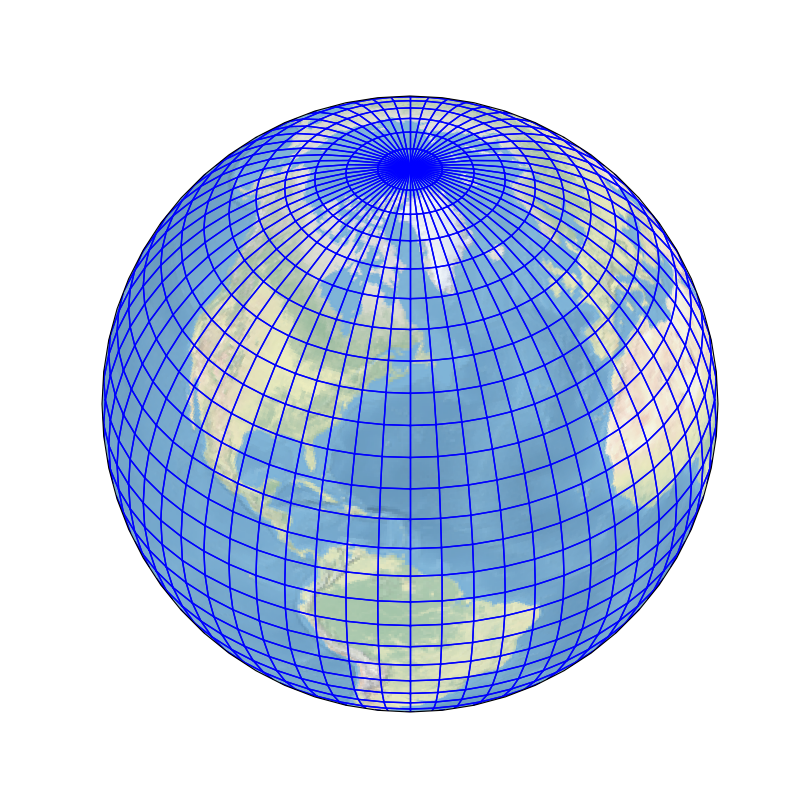
\includegraphics[width = \linewidth]{latlon_sphere}
		\caption{Latitude-longitude grid}\label{latlon-grid}
	\end{subfigure}%
  \hspace{1em}% Space between image A and B
\begin{subfigure}{.3\linewidth}
	\centering
	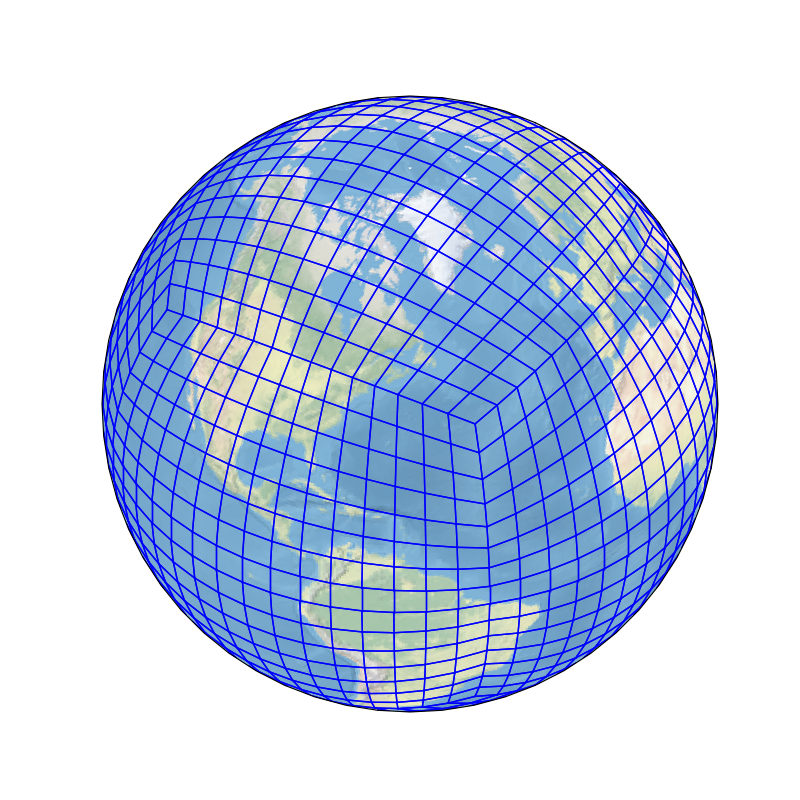
\includegraphics[width = \linewidth]{gnomonic_equiangular_15_sphere}
	\caption{Cubed-sphere}\label{cs-grid}
\end{subfigure}%
	\hspace{2em}% Space between image B and C
	\begin{subfigure}{.3\linewidth}
		\centering
		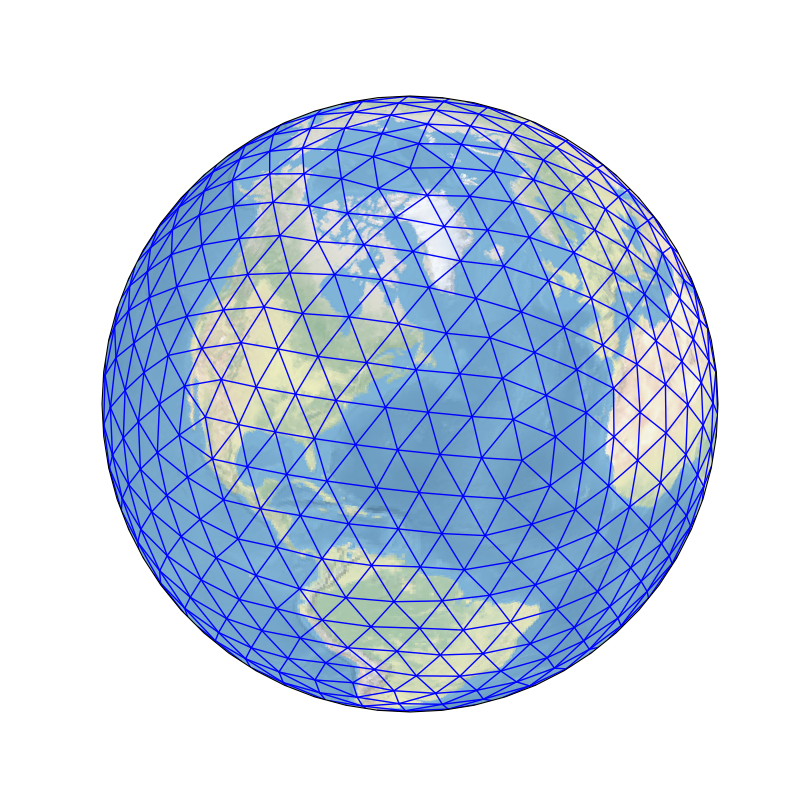
\includegraphics[width = \linewidth]{icos_pol_nopt_3_edsphere}
		\caption{Icosahedral grid}\label{icos-grid}
	\end{subfigure}
	\begin{subfigure}{.3\linewidth}
		\centering
		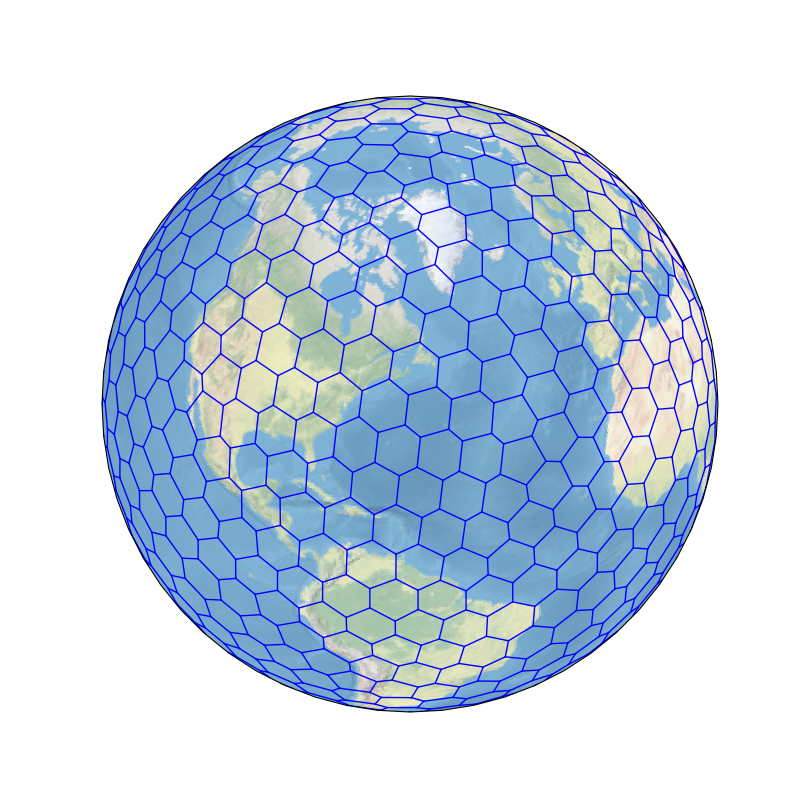
\includegraphics[width = \linewidth]{icos_pol_nopt_3_edhxsphere}
		\caption{Pentagonal/Hexagonal grid}\label{voronoi-grid}
	\end{subfigure}
	\begin{subfigure}{.3\linewidth}
		\centering
		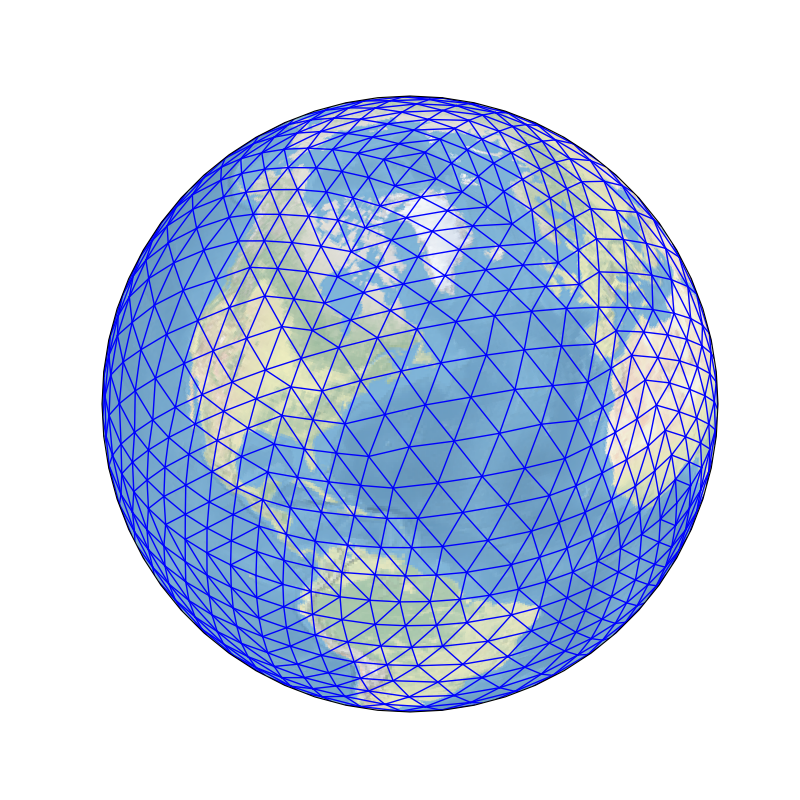
\includegraphics[width = \linewidth]{octg_pol_nopt_4_edsphere}
		\caption{Octahedral grid}\label{octg-grid}
	\end{subfigure}
	\caption{Examples of spherical grids: latitude-longitude grid (a) and grids based on Platonic solids (b)-(d).}
\end{figure}

The emergence of the Fast Fourier Transform (FFT) in the 1960s with the work from 
\citet{cooley:1965} allowed the computation of discrete Fourier transforms with
$N\log(N)$ complexity. 
The viability of the usage of FFTs for solving atmospheric flows was shown by \citet{orszag:1970},
using the barotropic vorticity equation on the sphere, and by \citet{eliasen:1970}, using
the primitive equations.
The spectral transform method expresses latitude-longitude grid values, that represent some scalar field,
using truncated spherical harmonics expansions, which consists of Fourier expansions 
in latitude circles and Legendre functions expansions in longitude circles. 
The coefficients in the spectral expansions are known
as spectral coefficients and are usually thought to live in the so-called spectral space.
Given the grid values, the spectral coefficients are obtained by performing a FFT followed by a 
Legendre Transform (LT). 
Conversely, given the spectral coefficients,
the grid values are obtained by performing an inverse LT followed by an inverse FFT.
The main idea of the spectral method is to apply the spectral transform, in order to 
go the spectral space, and evaluate spatial derivatives in the spectral space, which
consists of multiplying the spectral coefficients by constants. 
Then, the method performs the inverse spectral transform
in order to get back to grid space, and the nonlinear terms are treated on the grid space
\citep{krishnamurti:2006}.

The spectral transform makes the use of SI-SL methods computationally cheap, 
since the solution to elliptic problems becomes easy, once the spherical harmonics are
eigenfunctions of the Laplacian operator on the sphere.
Therefore, the spectral transform method gets faster when combined with the SI-SL approach
due to the larger times-steps allowed in this case.
Due to these enhancements, the spectral transform dominated global atmospheric modeling 
\citep{randall:2018} since the 1980s.
Indeed, the spectral method is still used in many current operational Weather Forecasting models such as
the Integrated Forecast System (IFS) from  European Centre for Medium-Range Weather Forecasts (ECMWF),
Global Forecast System (GFS) from National Centers for Environmental Prediction (NCEP) and the
Brazilian Global Atmospheric Model (BAM) \citep{figueroa:2016} from  Center for Weather Forecasting 
and Climate Research [Centro de Previsão de Tempo e Estudos Climáticos (CPTEC)].

With the beginning of the multicore era in the 1990s, the global atmospheric models
started to move towards parallel efficiency aiming to run at very high resolutions. 
Even though the spectral transform expansions have a global data dependency, some parallelization
is feasible among all the computations of FFTs, LTs and their inverses \citep{barros:1995}.
However, the parallelization of the spectral method requires data transpositions in order
to compute FFTs and LTs in parallel.  
These transpositions demand a lot of global communication using, for instance,
the Message Passing Interface (MPI) \citep{zheng:2018}. 
Indeed, the spectral transform becomes the most expensive component of global spectral models
when the resolution is increased due to the amount of MPI communications \citep{mueller:2019}.

The adiabatic and frictionless continuous equations that govern the atmospheric flow have 
conserved quantities. Among them, some of the most important are mass, total energy, 
angular momentum and potential vorticity \citep{thuburn:2011}.
Numerical schemes that are known for having discrete analogous of these conservative properties
are known as mimetic schemes.
As we pointed out, Semi-Lagrangian schemes lack mass conservation. Nevertheless, 
these schemes have been employed in dynamical cores for better computational performance.
However, dynamical cores should have discrete analogous of the 
continuous conserved quantities, especially concerning for longer simulation runs.

Aiming for better performance in massively parallel computers and conservation properties, 
new dynamical cores have been developed since the beginning of the 2000s.
Novel spherical grids have been proposed, in order to avoid the pole problem.
A popular choice are grids based on Platonic solids \citep{stan:2012}.
The construction of these grids relies on a Platonic circumscribed on the sphere and 
the projection of its faces onto the sphere, which leads to quasi-uniform and more isotropic
spherical grids.
Some examples of spherical grids based on Platonic solids employed in the new generation
of dynamical cores are the cubed-sphere (Figure \ref{cs-grid}), icosahedral grid (Figure \ref{icos-grid}), 
the pentagonal/hexagonal or Voronoi grid (Figure \ref{voronoi-grid}) and octahedral grid (Figure \ref{octg-grid}),
which are based on the cube, icosahedron, dodecahedron and octahedron, respectively \citep{ullrich:2017}.

\section{Motivations and the FV3 dynamical core}
The cubed-sphere became a popular quasi-uniform grid for the new generation of dynamical cores.
It was originally proposed by \citet{sadourny:1972} and it was revisited by \citet{ronchi:1996}.
Some of the cubed-sphere advantages are: uniformity; quadrilateral structure, 
making the grid indexing trivial; no overlappings; it is cheap to generate.
However, the major drawbacks of the cubed-sphere are: non-orthogonal coordinate system, which
leads to metric terms on the differential operators; discontinuity of the coordinate system
at the cube edges, which may generate numerical noise and
demands special treatment of discrete operators at the cube edges.

Despite of its drawbacks, the cubed-sphere has been adopted in some of the new generation
dynamical cores.
For instance, the cubed-sphere is used in the 
Community Atmosphere Model (CAM-SE) from the NCAR using spectral elements \citep{dennis:2012} and in the
Nonhydrostatic Unified Model of the Atmosphere (NUMA) from the US Navy using Discontinuous Galerkin 
methods \citep{giraldo:2013}. The cubed-sphere was also chosen to be used in the next UK Met Office
global model using mixed finite elements \citep{melvin:2022}.
At last, the Finite­ Volume Cubed-Sphere dynamical core (FV3) from the Geophysical Fluid 
Dynamics Laboratory (GFDL) and the National Oceanic and Atmospheric Administration (NOAA)
\citep{putman:2007,harris:2013} is another example
of new generation dynamical core based on the cubed-sphere.

The FV3 dycore is an extension of the Finite-Volume dycore (FVcore)
from latitude-longitude grids to the cubed-sphere.
The numerical methods from FVcore started to be developed with the advection scheme from the work \citet{lin:1994},
which is based on the piecewise linear scheme from \citet{vanleer:1977}. 
This scheme was later improved, using the Piecewise Parabolic Method (PPM) \citep{colella:1984, carpenter:1990}
using dimension splitting techniques that guarantee monotonicity and mass conservation,
for the advection equation \citep{lin:1996} and the shallow-water equations \citep{lin:1997}. 
An important feature is that the FVcore combines the  Arakawa C- and D-grids \citep{arakawa:1977},
where the C-grid values are computed in and intermediate time step. 
The full global model was then presented by \citet{lin:2004}.

A computational disadvantage of the FVcore is its Semi-Lagrangian formulation that creates more demand
for MPI communication when computing the accumulated fluxes \citep{lin:1996}.
The FVcore was then adapted to the cubed-sphere grid \citep{putmanthesis:2007, putman:2007}, 
to reach better performance in parallel computers, leading to the FV3 dycore.
Later, the FV3 also was improved to allow locally refinement grids 
through grid-nesting or grid-stretching \citep{harris:2013}.

Currently, the FV3 dycore is capable of perfoming hydrostatic and non-hydrostatic atmospheric simulations 
and it was chosen as the new US global weather prediction model, indeed, it replaced the spectral transform
Global Forecast System (GFS) in June, 2019
(\url{https://www.noaa.gov/media-release/noaa-upgrades-us-global-weather-forecast-model}, last accessed on March 19th, 2024).
Additionally, the FV3 dynamical core is employed in the GEOS Chem model \citep{martin:2022} from Harvard University, 
in NASA’s next-generation Mars Climate Model \citep{wilson:2022}, 
and also in the System for High-resolution prediction on Earth-to-Local Domain (SHiELD) model from GFDL \citep{harris:2020}.

However, a well-known problem that occurs on cubed-sphere models that use low-order numerical methods
is the grid imprinting visible due to the coordinate system discontinuity, 
especially at larger scales, leading to the emergence of a wavenumber 4 pattern.
This was reported in the paper of \citet{rancic:2017}, where the authors employ a 
finite-difference numerical scheme on the Uniform Jacobian cubed-sphere using a Arakawa B-grid.
The unpublished report from \citet{whitaker:2015} shows grid imprinting in other models, including 
the FV3.
More recently, \citet{mouallem:2023} has shown some idealized simulations using FV3 where grid imprinting appears in many simulations.
Generally speaking, grid imprinting refers to the presence of artificial behaviors in the numerical solution that are associated with the grid used.
It is important to emphasize that other quasi-uniform grids may also experience grid imprinting, such as hexagonal grids \citep{weller:2012, peixoto:2013, peixoto:2016}.

Despite being chosen as the new US global weather prediction model, there is a lack of numerical studies on the FV3 discretizations in the literature.
Numerical results for the advection equation on the cubed-sphere using the FV3 dynamical core were presented in \citet{putman:2007}.
However, they utilized extrapolations near the cube edges instead of the duo-grid approach from \citet{mouallem:2023}, which affects the convergence of this method.
The current solver of FV3 solves the shallow-water equation on the so-called Lagrangian surfaces.
This shallow-water solver, based on \citet{lin:1997}, 
utilizes the advection solver from \citet{putman:2007} to update the pressure, vorticity, and kinetic energy fluxes.
%Although \citet{mouallem:2023} present results on the convergence of some shallow-water tests,
%they do not provide a detailed discussion on the solver on the cubed-sphere itself.
Therefore, advection is a key aspect of the FV3 dynamical core, deserving better understanding. 
In this thesis, we propose to thoroughly examine all the minor details of the scheme from \citet{putman:2007} and suggest potential improvements, 
thereby addressing gaps in the existing literature.


\section{Outline and contributions}
This thesis is outlined as follows.
\begin{itemize}
\item Chapter \ref{chp-1d-fv} is dedicated to reviewing the Piecewise Parabolic Method (PPM) for the one-dimensional advection equation. 
In this Chapter, we demonstrate how the temporal component of PPM can be expressed as a departure point calculation. 
Subsequently, we enhance the departure point calculation from first-order (which is utilized in FV3) to second-order.
This enhancement results in a significant improvement, particularly in non-constant wind simulations.
Its benefits are also observed when using the monotonic version of PPM used in FV3 and proposed by \citet{lin:2004}.
The additional cost is only due to linear interpolation, which has little impact on the overall performance.

\item Chapter \ref{chp-2d-fv} reviews the dimension splitting method, which allows us to use one-dimensional methods, 
such as the PPM, to solve the two-dimensional advection equation. 
We review the current 2D advection scheme of FV3 on the plane proposed by \citet{putman:2007}.
The main feature of this scheme is that it preserves a constant scalar field when the wind is divergence-free.
We show through some numerical simulations that this scheme is second-order accurate only for divergence-free winds.
When the wind is not divergence-free, we show that this scheme is only first-order accurate.
On the other hand, we propose a small modification of the \citet{putman:2007} scheme 
using the second-order departure point computation presented in Chapter \ref{chp-1d-fv},
which allows us to achieve second-order accuracy and smaller errors for both divergent and divergence-free winds. 
Despite this scheme not preserving a constant scalar for divergence-free winds, it still exhibits second-order error in this case as well. 
Furthermore, when the monotonic scheme is used in the 1D solver, this scheme also has smaller errors compared to the \citet{putman:2007} scheme.

\item In Chapter \ref{chp-cs-grids}, we introduce the cubed-sphere grid utilized in FV3, 
which includes the equi-edge \citep{chen:2021} and equiangular grids \citep{ronchi:1996}, 
and we investigate their geometrical properties.
Next, we present all the tools necessary to extend the advection schemes on the plane from Chapter \ref{chp-2d-fv} to the sphere.
We review the contravariant/covariant wind formulation induced by the cubed-sphere mappings.
Additionally, we demonstrate how stencils can be computed near the cube-edges through the duo-grid 
technique to generate the ghost cells required for utilizing 1D Lagrange interpolation to fill these ghost cells.


\item Chapter \ref{chp-cs-fv} extends the ideas of Chapter \ref{chp-2d-fv} to the cubed-sphere grid using the tools from Chapter \ref{chp-cs-grids}.
The dimension-splitting method on each cubed-sphere panel works as in the plane, 
with the addition of metric terms due to the non-orthogonality of the grid and interpolation between panels to obtain ghost cell values needed for stencil computations. 
We show that the scheme from \citet{putman:2007} uses a less accurate formulation of the metric term to preserve the constant scalar for a divergence-free wind,
while our new scheme may use a more accurate formulation of the metric term, as it does not have this preservation constraint. 
The results are essentially the same as those from Chapter \ref{chp-2d-fv}, 
showing that our scheme successfully extends from the plane to the cubed-sphere and is more accurate. 
We also demonstrate that our new scheme has smaller errors at the corners compared to the scheme from \citet{putman:2007}.

\item In Chapter \ref{chp-cs-swm}, we present in detail the shallow-water solver of FV3
based on the extension of the solver by \citet{lin:1997} to the cubed-sphere.
This solver uses finite-volume advection fluxes to compute all operators.
Then, we may use our advection scheme introduced in Chapter \ref{chp-cs-fv} 
to compute the fluxes and compare the results with the scheme by \citet{putman:2007}.
We show that our scheme may help to slightly reduce the maximum errors for the geostrophic balanced case.
Additionally, we analyze the runtimes and show that our scheme adds a very small extra computational cost.
\end{itemize}

In summary, the main contribution of this thesis is a modified version of the two-dimensional scheme proposed by \citet{putman:2007}, which exhibits improved accuracy.
We give some final thoughts and future work perspectives in Chapter \ref{chp-conclusions}.